\chapter{Semejanza de Triángulos}

\rule{\textwidth}{0.1mm}
\begin{act}
	Construir en geogebra un lado $AB$ y luego construir otro lado $CD$ que sea el triple que este (Mejor si logra crear un deslizador para el valor de la razón incluso si logra crear un deslizador).
\end{act}
\rule{\textwidth}{0.1mm}

Observen laA siguiente figura

\begin{figure}[H]
	\centering
	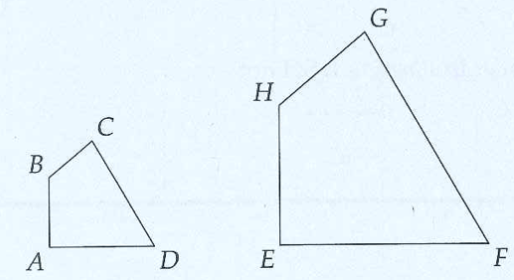
\includegraphics[width=0.7\linewidth]{Geometria/imgs/aops_geo_cuadrilateros_semejates}
	\caption{Dos cuadriláteros Semejantes}
	\label{semejanza_cuadrilateros}
\end{figure}



Podemos empezar a comparar lados, como? 

Si tu edad es 15 y la mía 30, pues $\frac{30}{15}=2$ es la cantidad de veces que mi edad supera a la tuya o \textbf{mi edad es el doble que la tuya} o \textbf{La razón entre nuestras edades es 2}. \textit{Y si yo tuviera 20 ? } : la razón entre ellas sería $\frac{20}{15}=\frac{4}{3}$.

Volviendo a nuestra figura \ref{semejanza_cuadrilateros}, \textit{Que creen que pasa con la razón entre los lados?} :  La razón entre \textbf{lados correspondientes} es la misma. Entonces en este caso 


\[
	\frac{AB}{EH} = \frac{BC}{HG} = \frac{CD}{GF} = \frac{DA}{FE}
\]

Se dice entonces que  $ABCD$ y $EFGH$ son semejantes esto es

\[ ABCD \sim EFGH
\]

\textbf{OJO.} Es importante el orden!

\rule{\textwidth}{0.1mm}
\begin{act}
	Construir en geogebra un triángulo $\triangle ABC$ y luego construir otro $\triangle YXZ$ que sea el triple que este (Mejor si logra que no importe si se mueven los vértices, se puede usar la herramienta segmento con longitud dada por ejemplo).
\end{act}
\rule{\textwidth}{0.1mm}

\begin{exer}{\ \\}
	\begin{enumerate} 
		\item (5.1.1 de \cite{Aops_Geometria}). Dados dos triángulos semejantes $\triangle ABC \sim \triangle YXZ$ cuáles de las siguientes afirmaciones son verdaderas?
		\begin{enumerate}[label=\Alph*)]
			\item $\frac{AB}{YC}=\frac{AC}{YZ}$
			\item$\frac{AB}{BC}=\frac{YX}{XZ}$
			\item $\frac{AB}{XZ}=\frac{BC}{YX}$
			\item $AC\cdot YX = YZ \cdot BA$
			\item $\frac{BC}{BA}=\frac{XY}{ZY}$
		\end{enumerate}
		\item  (5.1.2 de \cite{Aops_Geometria}). Si $\triangle ABC \sim \triangle ADB$, $AC=4cm$ y $AD=9cm$. Cuánto mide $AB$?
	\end{enumerate}
\end{exer}


\begin{theorem} \textbf{(Semejanza AA)}
	Si dos triángulos tienen dos ángulos correspondientes iguales, entonces los triángulos son semejantes. 
	\begin{figure}[H]
		\centering
		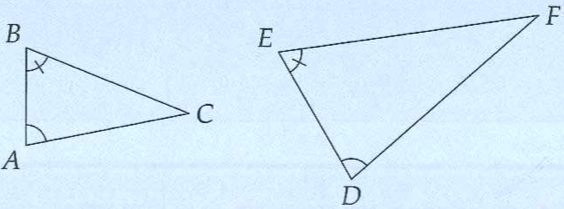
\includegraphics[width=0.7\linewidth]{Geometria/imgs/aops_geo_AA_semejanza}
		\caption{$\triangle ABC \sim \triangle DEF$ por el criterio de semejanza AA. }
		\label{teorema_aa_triangulossemejantes}
	\end{figure}
	Como $\angle A = \angle D$ y $\angle B = \angle E$ entonces $\triangle ABC \sim \triangle DEF$ y por tanto
	\[
		\frac{AB}{DE}=\frac{AC}{DF}=\frac{BC}{EF}
	\]
\end{theorem}

La demostración de este Teorema se verá mas adelane, ahora se puede ver en que problemas y cómo podemos usarlo.
\newpage




\begin{center}
	\vspace{-1cm}
	\section{ Ejercicios: Semejanza AA}
\end{center}

\begin{enumerate}
	\item \label{50_60_LAL} (5.2 de \cite{Aops_Geometria}). En la Figura \ref{semejanza5060ala}, encontrar las razones $\frac{AB}{DF}$, $\frac{AC}{DE}$, $\frac{BC}{EF}$ midiendi con una regla
	\begin{figure}[htbp]
		\centering
		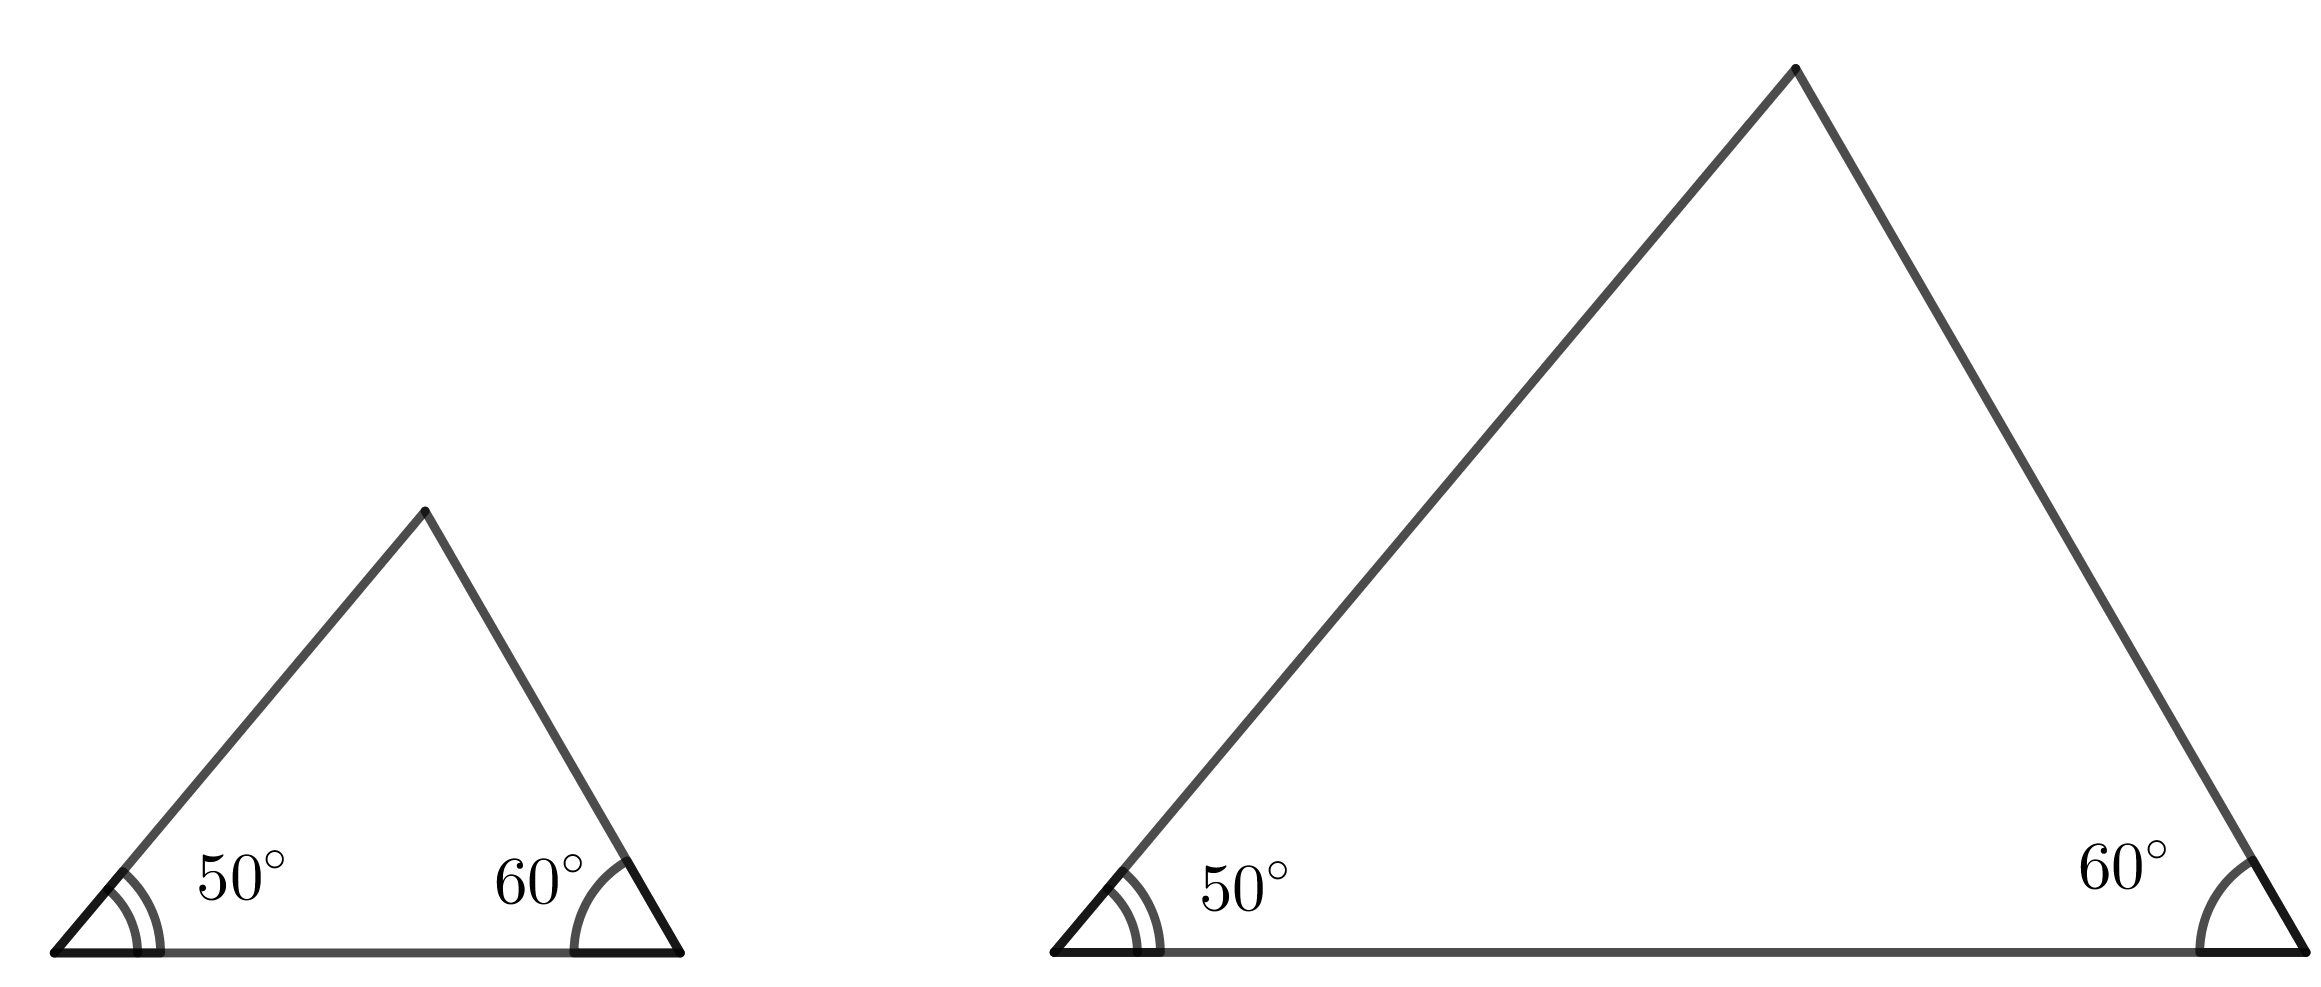
\includegraphics[width=0.7\linewidth]{Geometria/imgs/Semejanza_50_60_ALA}
		\caption{Figura del Problema \ref{50_60_LAL}. }
		\label{semejanza5060ala}
	\end{figure} 
\item (5.3 de \cite{Aops_Geometria}). El criterio AA servirá para cuadriláteros? Es decir, si $ABCD$ y $EFGH$ tienen los mismos ángulos entonces son semejantes? Si o no? Por qué?

\item \label{p5_4_aops_geo}(5.4 de \cite{Aops_Geometria}). Encontrar $MN$ (ver Figura \ref{aops_geo_p5_4} )
	\begin{figure}[H]
		\centering
		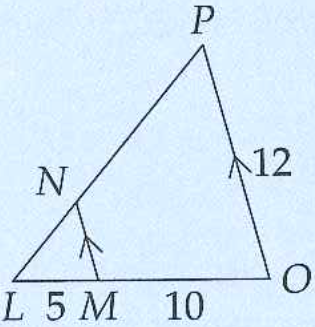
\includegraphics[width=0.25\linewidth]{Geometria/imgs/aops_geo_p5_4}
		\caption{Problema del ejercicio \ref{p5_4_aops_geo}}
		\label{aops_geo_p5_4}
	\end{figure}

\item ( p.310 de \cite{clemens}). Resolver los siguientes ejercicios


	\begin{figure}[th]
		\centering
		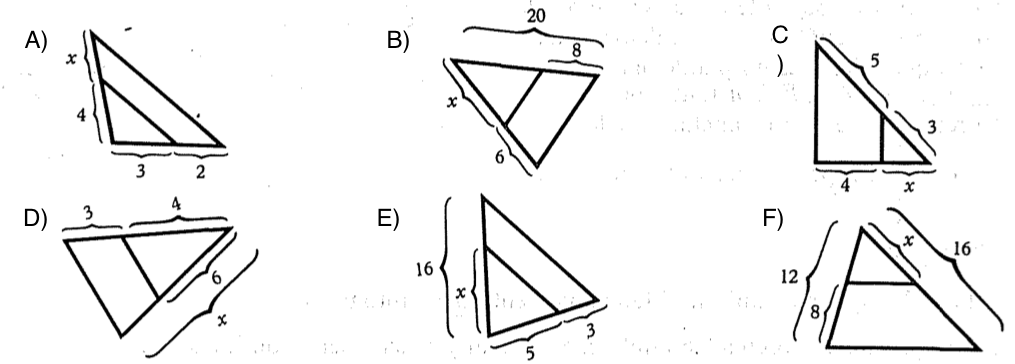
\includegraphics[width=0.87\linewidth]{Geometria/imgs/clemens_p310_3to8.png}
		\caption{}
		\label{clemens_p310_3to8}
	\end{figure}

\item \label{p5_5_aops_geo}(5.5 de \cite{Aops_Geometria}) Hallar $PY$ y $WX$ (ver Figura \ref{aops_geo_p5_5} )
	\begin{figure}[H]
		\centering
		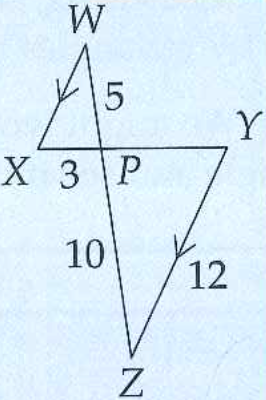
\includegraphics[width=0.25\linewidth]{Geometria/imgs/aops_geo_p5_5}
		\caption{Problema del ejercicio \ref{p5_5_aops_geo}}
		\label{aops_geo_p5_5}
	\end{figure}

\item \label{p5_6_aops_geo}(5.6 de \cite{Aops_Geometria}) Hallar $BC$ y $DC$ (ver Figura \ref{aops_geo_p5_6} )
\begin{figure}[H]
	\centering
	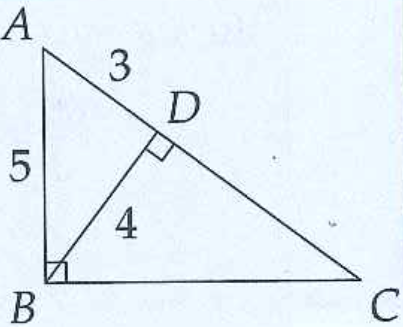
\includegraphics[width=0.25\linewidth]{Geometria/imgs/aops_geo_p5_6}
	\caption{Problema del ejercicio \ref{p5_6_aops_geo}}
	\label{aops_geo_p5_6}
\end{figure}

\item (UIS Clasificatoria Avanzado 2013) 
	\begin{figure}[H]
		\centering
		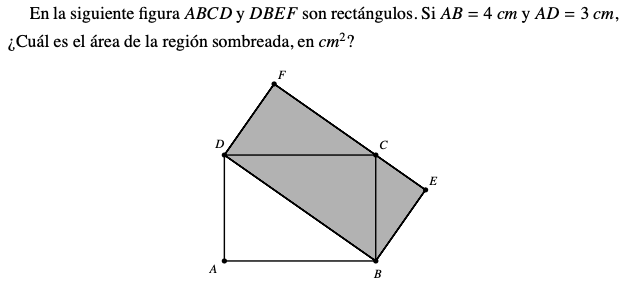
\includegraphics[width=0.9\linewidth]{Geometria/imgs/uis_2013_casi_avanzado}
		%\caption{}
		\label{uis_2013_casi_avanzado.png}
	\end{figure}
\end{enumerate}
\newpage

\begin{theorem}
	\label{teorema_paralela_en_un_triangulo}En un triángulo $\triangle ABC$, si $D$ y $E$ están entre $AB$ y $BC$ respectivamente y además $DE||AC$, entonces
	 \begin{equation*}
		\frac{AD}{DB}=\frac{EC}{BE}
	 \end{equation*}	 	
	Es decir la paralela divide a los lados proporcionalmente. 
\end{theorem}

\textbf{\textit{Esto para qué?}}
\begin{ejemplo}
	\label{ejemplo_dividir_lado_e_tres}
	Dado un segmento, solamente usando regla (sin medir) y compás dividir un segmento en 5 partes iguales.
	
	\begin{figure}[H]
		\centering
		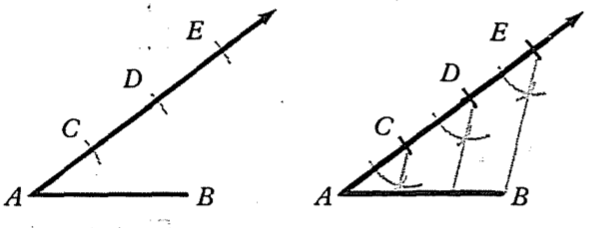
\includegraphics[width=0.7\linewidth]{Geometria/imgs/clemens_dividir_lado_en_tres}
		\caption{Ejemplo \ref{ejemplo_dividir_lado_e_tres}}
		\label{clemens_dividir_lado_en_tres}
	\end{figure}
	
\end{ejemplo}

\textit{Para probar la reciproca del Teorema \ref{teorema_paralela_en_un_triangulo} ver antes este ejemplo:}

\begin{ejemplo}\label{Ejemplo_aops_p_5_9}
	(5.9 de \cite{Aops_Geometria}) En la Figura \ref{aops_geo_p_5_9}, se tiene que 
	\[
		\frac{AB}{AC} = \frac{AD}{AE} = \frac{4}{5},
	\]
	probar que $BD||CE$.\\
	\textbf{Rta:} Note que si $BD||CE$ ya está por criterio AA. Suponiendo un segmento $BX||CE$ se puede llegar a que $AX=12$ y por tanto $X$ es $D$ y así $BD||CE$.
	
	
	\begin{figure}[H]
		\centering
		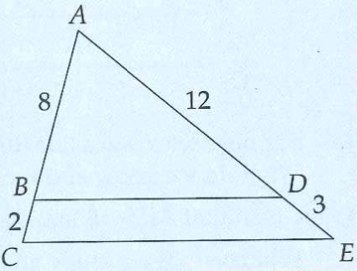
\includegraphics[width=0.5\linewidth]{Geometria/imgs/aops_geo_p_5_9}
		\caption{Figura del ejemplo \ref{Ejemplo_aops_p_5_9}.}
		\label{aops_geo_p_5_9}
	\end{figure}
\end{ejemplo}







Con el anterior ejemplo se pueden intentar probar el siguiente teorema.

\begin{theorem}
	(Reciproca del Teorema \ref{teorema_paralela_en_un_triangulo} ). En un triángulo $\triangle ABC$, si $D$ y $E$ están entre $AB$ y $BC$ respectivamente tal que
	\begin{equation*}
	\frac{AD}{DB}=\frac{EC}{BE}
	\end{equation*}	 	
	entonces $DE||AC$. 
\end{theorem}


\begin{ejemplo}{(5.6 de \cite{Aops_Geometria}). \\}
	\item \label{p5_7_aops_geo} Probar que $\frac{EY}{EX} = \frac{AD}{DB}$ (ver Figura \ref{aops_geo_p5_7} )
	\begin{figure}[H]
		\centering
		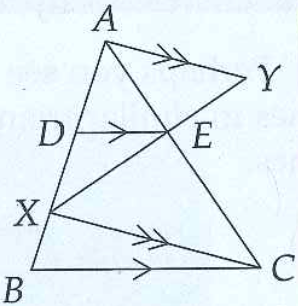
\includegraphics[width=0.25\linewidth]{Geometria/imgs/aops_geo_p5_7}
		\caption{Problema del ejermplo \ref{p5_7_aops_geo}}
		\label{aops_geo_p5_7}
	\end{figure}
	
\end{ejemplo}

\begin{exer}{\ \\}
	\item Realizar las siguientes actividades (tomadas de \cite{clemens}) menos el 15,16 y las actividades del final.
	
		\setlength{\voffset}{0cm}
		\setlength{\hoffset}{-1cm}
		
		\includepdf[pages=328,pagecommand={},width=1\textwidth]{/Users/juanolmos/MEGA/Olimpiadas/Libros/GEOMETRIA_CLEMENS_FINALLL.pdf}
		
		\setlength{\voffset}{0cm}
		\setlength{\hoffset}{-1cm}
		
		\includepdf[pages=329,pagecommand={},width=1\textwidth]{/Users/juanolmos/MEGA/Olimpiadas/Libros/GEOMETRIA_CLEMENS_FINALLL.pdf}
		
		\setlength{\voffset}{0cm}
		\setlength{\hoffset}{-1cm}
		
		\includepdf[pages=330,pagecommand={},width=1\textwidth]{/Users/juanolmos/MEGA/Olimpiadas/Libros/GEOMETRIA_CLEMENS_FINALLL.pdf}

\end{exer}


\newpage
\begin{center}
	\vspace{-1cm}
	\section{ Ejercicios: Semejanza AA}
\end{center}

\begin{exer}{\ \\}	
\begin{enumerate}
	\item (5.2.1 de \cite{Aops_Geometria}) Realizar los siguientes ejercicios 
	\begin{enumerate}[label=\Alph*)]
		 \item Hallar $AC$ y $BC$ en la Figura A) .
		
		\item  Hallar $HJ$ en la Figura B) .
		
		\item  Hallar $ON$ y $MN$ en la Figura C).
		
		\item Hallar $RS$ en la Figura D) .
		
			\begin{figure}[H]
				\centering
				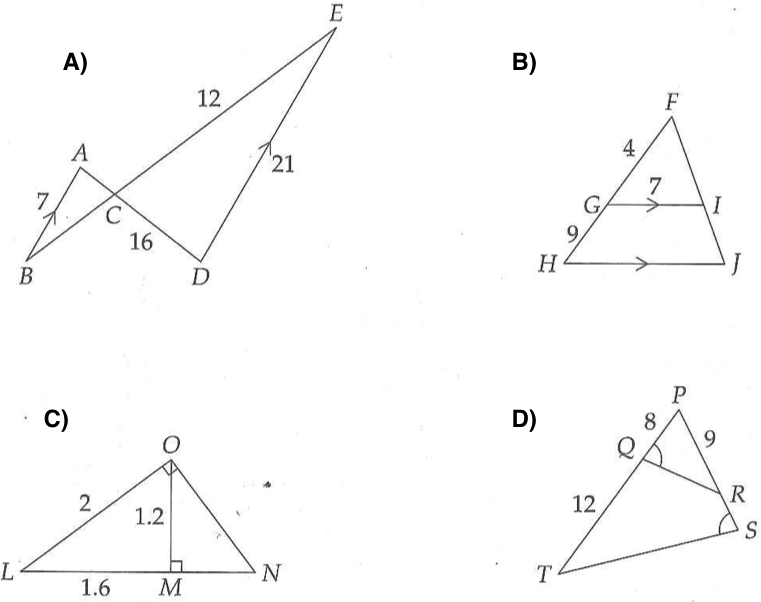
\includegraphics[width=0.7\linewidth]{Geometria/imgs/aops_geo_5_2_1}
				%\caption{Problema}
				\label{aops_geo_5_2_1}
			\end{figure}
	\end{enumerate}
	
	\item \label{p_5_2_3_aopgeo}(5.2.3 de \cite{Aops_Geometria}) En la Figura \ref{aops_geo_5_2_3} $WXYZ$ es un cuadrado. $M$ es punto medio de $YZ$ y $AB\bot MX$.
		\begin{figure}[H]
			\centering
			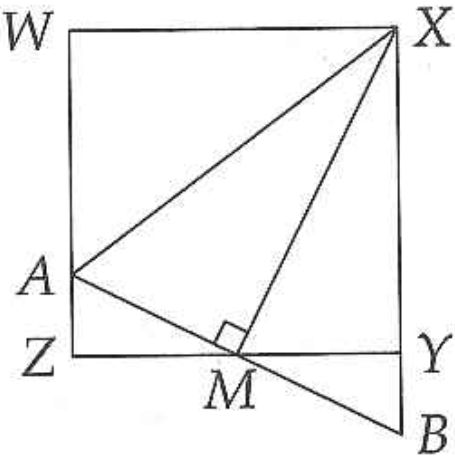
\includegraphics[width=0.3\linewidth]{Geometria/imgs/aops_geo_5_2_3}
			\caption{Problema \ref{p_5_2_3_aopgeo} }
			\label{aops_geo_5_2_3}
		\end{figure}

	
	\begin{enumerate}[label=\Alph*)]
		\item Mostrar que $WZ||XY$.
		\item Probar que $AZ=YB$.
		\item Probar que $XB=XA$.
		\item Probar que $\triangle AZM\sim \triangle MYX$ y usar esto para probar que $AZ=\frac{1}{4} XY$.
	\end{enumerate}

	\item (5.2.4 de \cite{Aops_Geometria}). En $\triangle ABC$, $AB=AC$, $BC=1$ y $\angle BAC = 36 \degree$. Sea $D$ sobre $AC$ tal que $\angle ABD = \angle CBD$.
	\begin{enumerate}[label=\Alph*)]
		\item Mostrar que $\triangle ABC\sim \triangle BCD$.
		\item\textbf{(Wow)} Hallar $AB$.
	\end{enumerate}
	
	\item \label{p_5_2_5_aopgeo} (5.2.5 de \cite{Aops_Geometria}) \textbf{Woow}. Encontrar $x$ en terminos de $y$ dado el diagrama de la Figura \ref{aops_geo_5_2_5}.
	\begin{figure}[H]
		\centering
		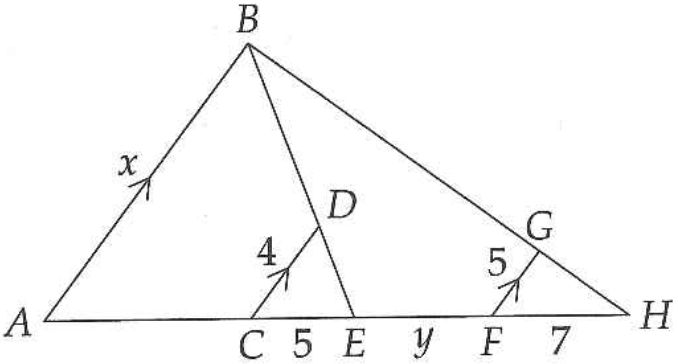
\includegraphics[width=0.5\linewidth]{Geometria/imgs/aops_geo_5_2_5}
		\caption{Problema \ref{p_5_2_5_aopgeo} }
		\label{aops_geo_5_2_5}
	\end{figure}
\end{enumerate}
	
\end{exer}

\newpage
\begin{ejemplo}
	\label{teorema_bisectriz}
	(\textbf{Teorema de la bisectriz}). En un $\triangle ABC$ al trazar la bisectriz de $\angle A $ esta intersecta al lado $BC$ en $D$ de forma que 
	\[
		\frac{AB}{AC}=\frac{BD}{DC}
	\].\\
	\textbf{Rta:} Prolongar la bisectriz hasta un punto $E$ de forma que $EC=AC$ y ver semejanzas.
\end{ejemplo}

\begin{ejemplo}
	\label{teorema_altura_en_triangulo_rectangulo}
	(\textbf{Teorema altura en un triángulo rectángulo}). Sea $\triangle ABC$ un triángulo rectángulo donde $\angle A= 90\degree $, sea $D$ la base de la altura del vértice $A$. Probar que
	\[
		BD\cdot DC = {AD}^2
	\]
	\textbf{Rta:} Ver la semejanza $\triangle ABC \sim \triangle DBA$. Otra solución es por pitágoras, ver ambas.
\end{ejemplo}

\section{Criterio LAL}
\begin{theorem} \textbf{(Semejanza LAL)}
	Si dos triángulos tienen dos lados corresponndientes proporcionales y además el ángulo entre ellos es el mismo entonces son semejantes. Es decir, si $\frac{AB}{DE} = \frac{AC}{DF}$ y $\angle A =\angle D$ entonces $\triangle ABC \sim \triangle DEF$ (Ver Figura \ref{aops_geo_criterio_LAL}).
	
	\begin{figure}[H]
		\centering
		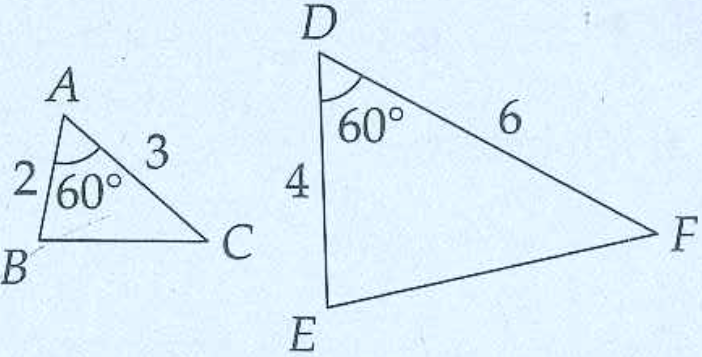
\includegraphics[width=0.5\linewidth]{Geometria/imgs/aops_geo_criterio_LAL}
		\caption{Criterio LAL}
		\label{aops_geo_criterio_LAL}
	\end{figure}
\end{theorem}

Mirar nuevamente el ejercicio \ref{aops_geo_p_5_9} y ver que $\triangle ABD \sim \triangle ACE$. \textit{Cómo se puede usar esto para probar el criterio LAL? } :Vea que sería como meter un triángulo dentro del otro.

\begin{ejemplo}
	(5.10 de \cite{Aops_Geometria} ). Hallar $BC$ si el perimetro de $\triangle BCD$ es 20 (Ver Figura \ref{aops_geo_p_5_10}).
\begin{figure}[H]\label{ej_p_5_10_aops}
	\centering
	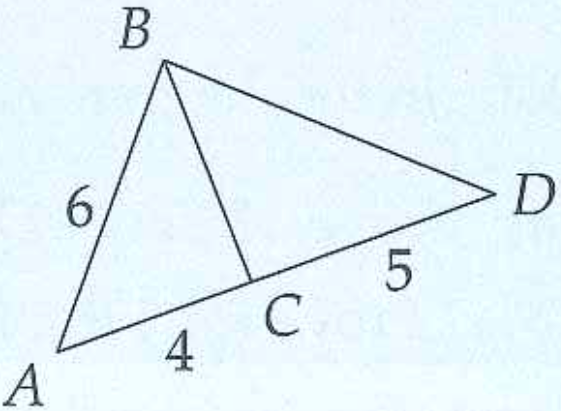
\includegraphics[width=0.3\linewidth]{Geometria/imgs/aops_geo_p_5_10}
	\caption{Ejemplo \ref{ej_p_5_10_aops}}
	\label{aops_geo_p_5_10}
\end{figure}
	\textbf{Rta:} Note que $\triangle ABC \sim \triangle ADB$ pues comparten $\angle A$ y $$\frac{AB}{AD}=\frac{AC}{AB}=\frac{2}{3},$$ entonces son semejantes por \textbf{LAL} y por tanto $\frac{BC}{BD}=\frac{2}{3}$, o sea $BC=\frac{2\cdot BD}{3}$ y así como el perimetro de $\triangle BCD=20$, entonces
	\begin{equation*}
		\begin{split}
			5+BD+BC&=20\\
			BD+\frac{2\cdot BD}{3} &= 15\\
			3BD+2BD&=45\\
			5BD&=45\\
			BD&=9,
		\end{split}
	\end{equation*}
			y así $BC=6$.
\end{ejemplo}

\rule{\textwidth}{0.1mm}
\begin{act}
	Construir en geogebra un triángulo $\triangle ABC$ y luego construir otro $\triangle YXZ$ usando el criterio LAL (Si se puede, usar deslizadores para variar la razón).
\end{act}
\rule{\textwidth}{0.1mm}

\newpage
\begin{center}
	\vspace{-1cm}
	\subsection{ Ejercicios: Semejanza LAL}
\end{center}

\begin{enumerate}
	\item \label{P531_aopgeo} (5.3.1 de \cite{Aops_Geometria}). Encontrar $DE$ en la Figura \ref{531_aopgeo}
	
		\begin{figure}[H]
			\centering
			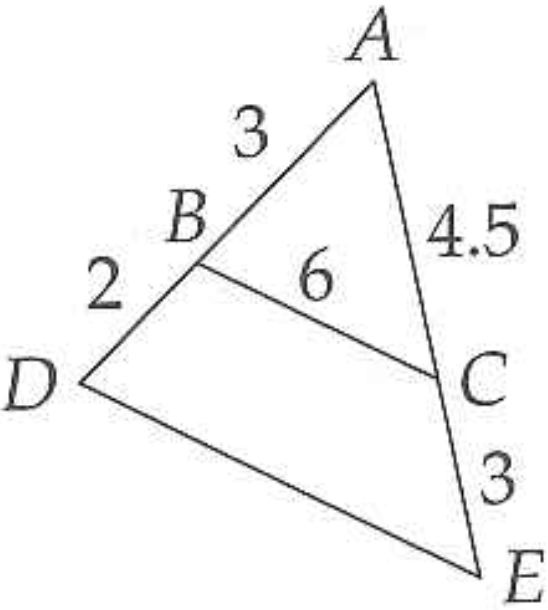
\includegraphics[width=0.2\linewidth]{Geometria/imgs/531_aopgeo}
			\caption{Ejercicio \ref{P531_aopgeo} }
			\label{531_aopgeo}
		\end{figure}
	
	\item \label{P532_aopgeo} (5.3.2 de \cite{Aops_Geometria}). En la Figura \ref{532_aopgeo}, $M$ es el punto medio de $\overline{EH}$ y $\overline{FG}$. $E$ y $F$ son puntos medios de $\overline{IM}$ y $\overline{MJ}$ respectivamente. Probar que $IJ||GH$.
	
	\begin{figure}[H]
		\centering
		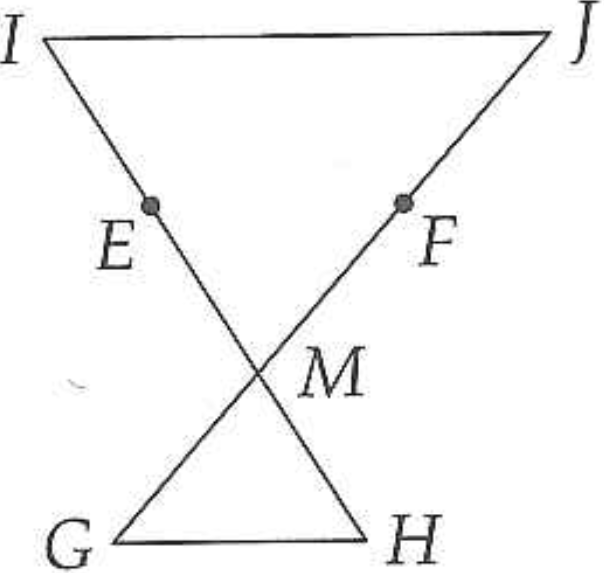
\includegraphics[width=0.25\linewidth]{Geometria/imgs/532_aopsgeo}
		\caption{Ejercicio \ref{P532_aopgeo} }
		\label{532_aopgeo}
	\end{figure}

	\item \label{P533_aopgeo} (5.3.3 de \cite{Aops_Geometria}). Mostrar que si ${WZ}^2 = (WX)(WY)$ en la Figura \ref{533_aopgeo}, entonces $\angle WZX = \angle WYZ$.
	
	\begin{figure}[H]
		\centering
		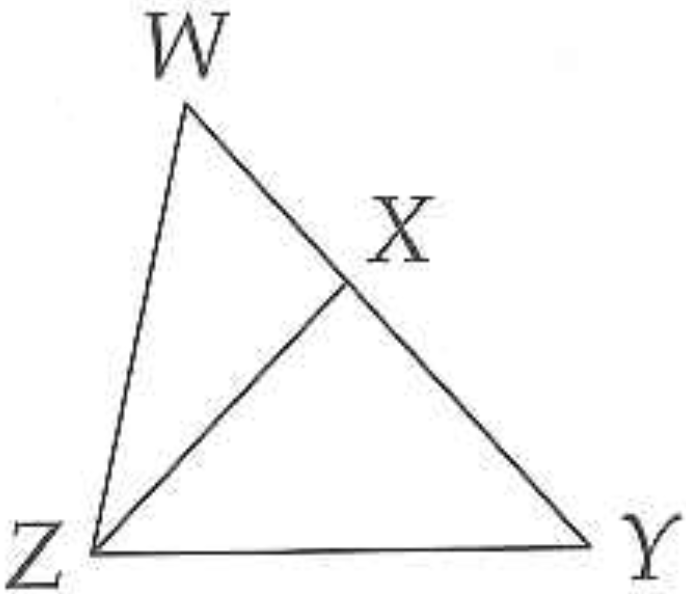
\includegraphics[width=0.25\linewidth]{Geometria/imgs/533_aopsgeo}
		\caption{Ejercicio \ref{P533_aopgeo} }
		\label{533_aopgeo}
	\end{figure}
	
	\item \label{P534_aopgeo} (5.3.4 de \cite{Aops_Geometria}). En la Figura \ref{534_aopgeo}, $\angle PRQ = \angle PQA = \angle 90\degree $, $QR=QA$ y $\angle QPC = \angle RPC$.
	\begin{enumerate}[label=\Alph*)]
			\item Probar $\angle QCB = \angle QBC$.
			\item \textbf{Wow}. Probar que $RA||PB$.
	\end{enumerate}
	
		\begin{figure}[H]
			\centering
			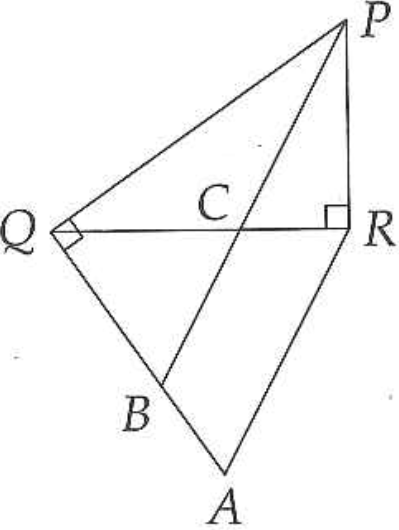
\includegraphics[width=0.25\linewidth]{Geometria/imgs/534_aopsgeo}
			\caption{Ejercicio \ref{P534_aopgeo} }
			\label{534_aopgeo}
		\end{figure}
	
	
\end{enumerate}
\newpage

\section{Criterio LLL}
\begin{theorem} \textbf{(Semejanza LLL)}
	Si dos triángulos tienen los lados corresponndientes proporcionales entonces son semejantes. Es decir, si $\frac{AB}{DE} = \frac{AC}{DF}= \frac{BC}{EF}$ entonces $\triangle ABC \sim \triangle DEF$ (Ver Figura \ref{aops_geo_criterio_LLL}).
	
	\begin{figure}[H]
		\centering
		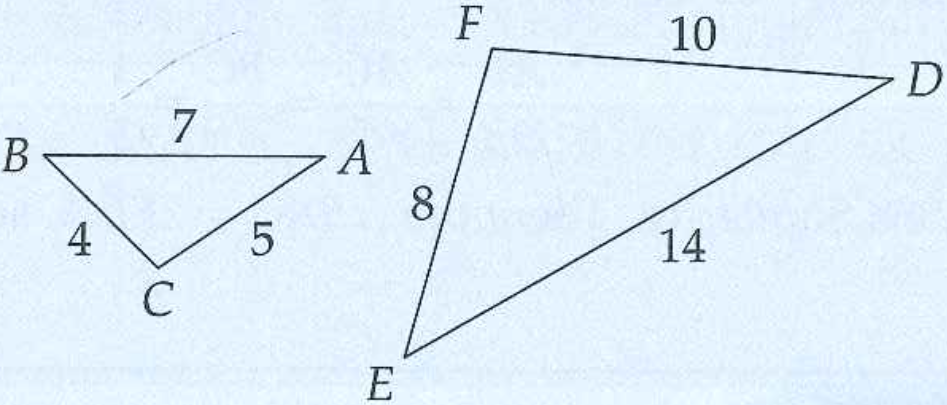
\includegraphics[width=0.5\linewidth]{Geometria/imgs/aops_geo_criterio_LLL}
		\caption{Criterio LLL}
		\label{aops_geo_criterio_LLL}
	\end{figure}
\end{theorem}

\begin{ejemplo}{(5.11 de \cite{Aops_Geometria})}
\label{ejemplo_5_11_aopsgeo}En la Figura \ref{5_11_aopsgeo} probar que $AE||BC$ y $AB||DE$.
	\begin{figure}[H]
		\centering
		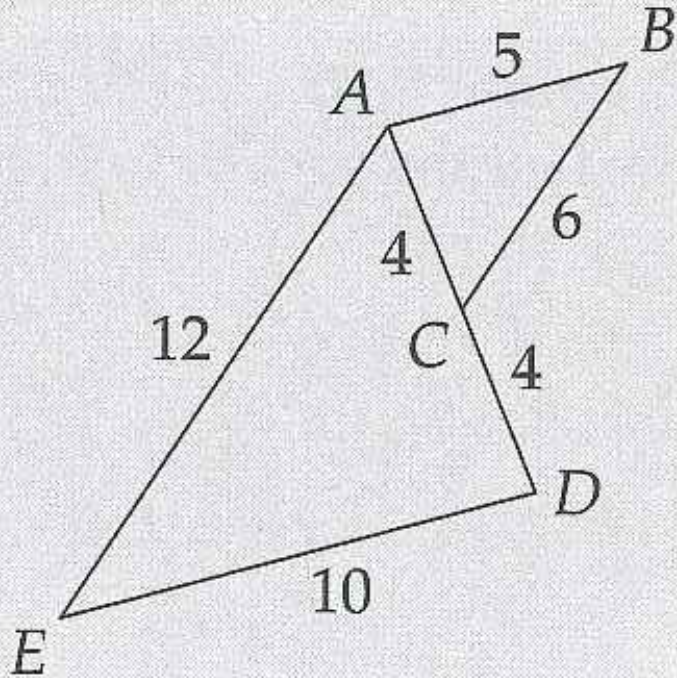
\includegraphics[width=0.3\linewidth]{Geometria/imgs/5_11_aopsgeo}
		\caption{Ejemplo \ref{ejemplo_5_11_aopsgeo}.}
		\label{5_11_aopsgeo}
	\end{figure}
		\textbf{Rta:} Para que $AE||BC$ se tiene que probar que $\angle EAD =\angle BCA$ y para probar que $AB||DE$ se tiene que probar que $\angle CAB =\angle AED$, y esto se tendría si $\triangle EAD \sim \triangle BCA$. Note que $\frac{EA}{BC}=\frac{12}{6}=2$, $\frac{ED}{BA}=\frac{10}{5}=2$ y $\frac{AD}{CA}=\frac{8}{4}=2$, es decir, son semejantes por \textbf{LLL}.
\end{ejemplo}


\begin{ejemplo}{(5.12 de \cite{Aops_Geometria})}
	\label{ejemplo_5_12_aopsgeo}En la Figura \ref{5_12_aopsgeo} se tiene que $DE||BC$. Encontrar $x,y,z$.
	\begin{figure}[H]
		\centering
		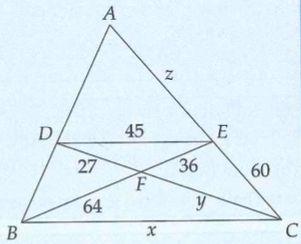
\includegraphics[width=0.3\linewidth]{Geometria/imgs/5_12_aopsgeo}
		\caption{Ejemplo \ref{ejemplo_5_12_aopsgeo}.}
		\label{5_12_aopsgeo}
	\end{figure}
		\textbf{Rta:} Con la semejanza $\triangle FED \sim \triangle FBC$ se pueden hallar $x$ e $y$. Y con la semejanza $\triangle AED \sim \triangle ACB$ se puede calcular $z$.
\end{ejemplo}

\begin{ejemplo}{(5.13 de \cite{Aops_Geometria})}
	\label{ejemplo_5_13_aopsgeo}En la Figura \ref{5_13_aopsgeo} se tiene que $AB=6$ y $AC=10$. Encontrar $AD$.
	\begin{figure}[H]
		\centering
		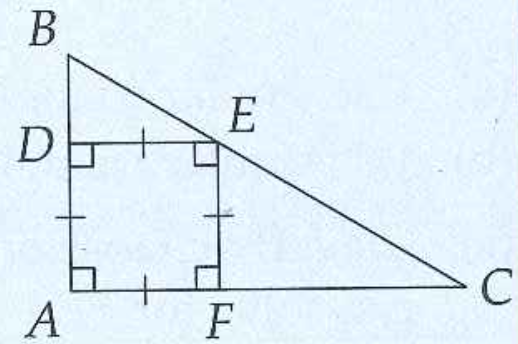
\includegraphics[width=0.3\linewidth]{Geometria/imgs/5_13_aopsgeo}
		\caption{Ejemplo \ref{ejemplo_5_13_aopsgeo}.}
		\label{5_13_aopsgeo}
	\end{figure}
	\textbf{Rta:} Dando un valor $x$ al lado del cuadrado y viendo que $\triangle BAC \sim \triangle BDE \sim \triangle EFC$.
\end{ejemplo}

\begin{ejemplo}{(5.14 de \cite{Aops_Geometria})}
	\label{ejemplo_5_14_aopsgeo}En la Figura \ref{5_14_aopsgeo} mostrar 
	\begin{enumerate}[label=\Alph*) ]
			\item ${PX}^2 = QX\cdot RX$.
			\item ${PR}^2 = RX\cdot RQ$.
			\item ${PQ}^2 = QX\cdot QR$.
	\end{enumerate}
	\begin{figure}[H]
		\centering
		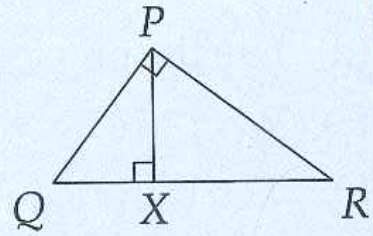
\includegraphics[width=0.3\linewidth]{Geometria/imgs/5_14_aopsgeo}
		\caption{Ejemplo \ref{ejemplo_5_14_aopsgeo}.}
		\label{5_14_aopsgeo}
	\end{figure}
\end{ejemplo}

\begin{ejemplo}{(5.15 de \cite{Aops_Geometria})}
	\label{ejemplo_5_15_aopsgeo} $\triangle ABC \sim \triangle XYZ$, $\frac{AB}{XY}=4$, y $\left[ABC\right]=64$. Hallar $\left[XYZ\right]$
	\textbf{Rta:} Sabemos que si dos triángulos son semejantes entonces las alturas tienen la misma proporción que esta semejanza. 
\end{ejemplo}

\begin{ejemplo}{(5.16 de \cite{Aops_Geometria})}
	\label{ejemplo_5_16_aopsgeo}En la Figura \ref{5_16_aopsgeo}, $P$ es el punto medio de $\overline{AB}$. Probar que $\overline{PQ}\parallel \overline{BC}$.
	\begin{figure}[H]
		\centering
		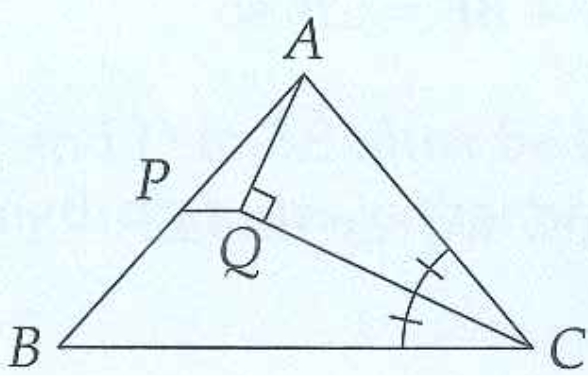
\includegraphics[width=0.3\linewidth]{Geometria/imgs/5_16_aopsgeo}
		\caption{Ejemplo \ref{ejemplo_5_16_aopsgeo}.}
		\label{5_16_aopsgeo}
	\end{figure}
	\textbf{Rta: }Si se extiende $AQ$ hasta intersectar a $BC$ en $H$, se puede ver $\triangle CQA \cong \triangle CQH$ entonces $AQ=QH$. Entonces como $\frac{AP}{AB}=\frac{AQ}{AH}=\frac{1}{2}$ entonces $\overline{PQ}\parallel \overline{BC}$ por el Teorema \ref{teorema_paralela_en_un_triangulo}.
\end{ejemplo}

\begin{ejemplo}{(5.17 de \cite{Aops_Geometria})}
	\label{ejemplo_5_17_aopsgeo}En la Figura \ref{5_17_aopsgeo}, El asta de bandera $\overline{CD}$ mide 12 metros de alto. El asta de bandera $\overline{AB}$ mide 9 metros de alto. Ambas astas son perpendiculares al piso. Un cable recto está amarrado desde $B$ hasta $D$ y otro desde $A$ hasta $C$. Las astas están separadas 40 metros y los cables se encuentran en $E$ que está justamente encima del punto $F$ que está en el piso. Hallar $EF$.
	\begin{figure}[H]
		\centering
		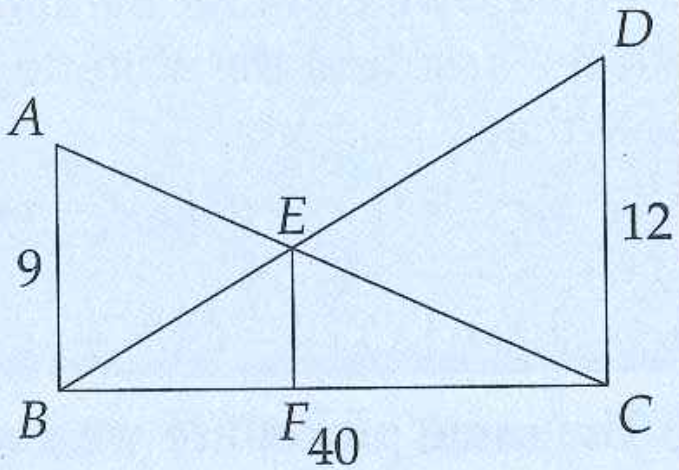
\includegraphics[width=0.3\linewidth]{Geometria/imgs/5_17_aopsgeo}
		\caption{Ejemplo \ref{ejemplo_5_17_aopsgeo}.}
		\label{5_17_aopsgeo}
	\end{figure}
	\textbf{Rta: }Note que $\triangle ABC \sim \triangle EFC$ y $\triangle DCB \sim \triangle EFB$. Opción 1, De forma algebraica tomando $EF=h$ y $FC=x$ y planteando las dos ecuaciones de la semejanza. Opción 2 no se usa que $BC=40$ \textbf{te atreves?}, de la semejanza se tiene que $$\frac{EF}{AB} = \frac{\textbf{FC}}{\textbf{BC}} = \frac{EC}{AC}\hspace{5mm}\text{ y }\hspace{5mm}\frac{EF}{DC} = \frac{\textbf{FB}}{\textbf{BC}} = \frac{EB}{DB}.$$
	Sumando las fracciones subrayadas 
	\begin{equation*}
		\begin{split}
			\frac{EF}{AB}  + \frac{EF}{DC} &= \frac{\textbf{FC}}{\textbf{BC}} + \frac{\textbf{FB}}{\textbf{BC}} \\
			\frac{EF}{AB}  + \frac{EF}{DC} &= 1 \\
			EF \left( \frac{1}{AB}  + \frac{1}{DC} \right) &=1\\
			EF \left( \frac{1}{9}  + \frac{1}{12} \right) &=1\\
			EF \frac{21}{108} &=1\\
			EF &= \frac{108}{21}\\
			EF  &= \frac{36}{7}
		\end{split}
	\end{equation*}
\end{ejemplo}

\begin{ejemplo}{(5.18 de \cite{Aops_Geometria})}
	\label{ejemplo_5_18_aopsgeo}En la Figura \ref{5_18_aopsgeo}, Hallar $BE$ y$DE$ \textbf{sin} usar el cirterio de semejanza semejanza AA.
	\begin{figure}[H]
		\centering
		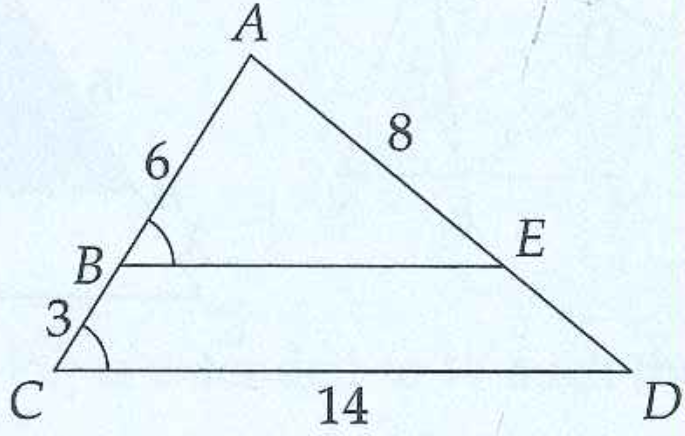
\includegraphics[width=0.5\linewidth]{Geometria/imgs/5_18_aopsgeo}
		\caption{Ejemplo \ref{ejemplo_5_18_aopsgeo}.}
		\label{5_18_aopsgeo}
	\end{figure}
	\textbf{Rta: }Queremos encontrar que relación relación $\frac{AB}{AC} = \frac{AE}{ED}$ es cierta. Una técnica útil es usar \textbf{áreas!} podemos trazar $BD$ y $CE$ (Ver figura \ref{5_18_aopsgeo_sol}) para construir triángulos que nos puedan dar esta información, pues note que la relación $\frac{AB}{AC}$ surge al comparar $[ABE]$ y $[ACE]$ ya que al tener la misma altura los triángulos $\triangle ABE$ y $\triangle ACD$, como $[ABE]=\frac{1}{2}AB\cdot h$, entonces $h=\frac{2[ABE]}{AB}$ y del $\triangle AEC$ se tiene que $h=\frac{2[ACE]}{AC}$, entonces 
	\[
		\frac{[ABE]}{[ACE]} = \frac{AB}{AC} =\frac{6}{9} = \frac{2}{3}
	\]
	Lo mismo se tiene con $\triangle ABE$ y $\triangle ABD$, tienen la misma altura y entonces 
	\[
	\frac{[ABE]}{[ABD]} = \frac{AE}{AD} =\frac{8}{8+ED} 
	\]
	\begin{figure}[H]
		\centering
		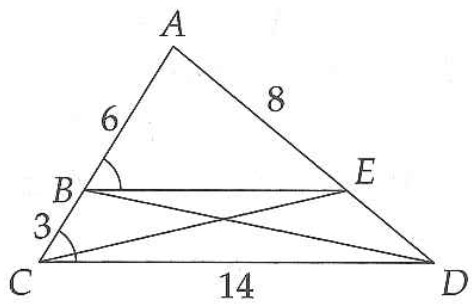
\includegraphics[width=0.5\linewidth]{Geometria/imgs/5_18_aopsgeo_sol}
		\caption{Solución de \ref{ejemplo_5_18_aopsgeo}}
		\label{5_18_aopsgeo_sol}
	\end{figure}
	Vemos entonces que si $\frac{AB}{AC} = \frac{AE}{ED}$ entonces ya podemos conocer $ED$. Necesitariamos entonces que $\frac{[ABE]}{[ACE]}=\frac{[ABE]}{[ABD]}$, es decir que $[ACE]=[ABD]$. Y esta igualdad es cierta porque se puede ver que $[BED]=[BEC]$ y como comparten $[ABD]$ entonces efectivamente $[ACE]=[ABD]$. Entonces $\frac{AB}{AC} = \frac{AE}{ED}$ y así $\frac{2}{3}=\frac{8}{8+ED} $, de donde $ED=4$.

		Para hallar $BE$ quisieramos aplicar algo parecido, entonces basta con mover el $\triangle ABE$ al vértice $D$, ver Figura \ref{5_18_aopsgeo_sol2}. Se puede ver $\triangle ABE \cong \triangle A'B'D$  para ver que $A'D=AE=8$ y que $\angle A' = \angle A$ y así tenemos el mismo problema cuando calculamos $DE$ pero girado y el problema es hallar $B'D$ pues sabemos por la congruencia que $B'D=BE$. De ese problema supimos que con solo áreas se puede probar que
		\[
			\frac{A'D}{AD} = \frac{B'D}{CD},
		\]
		es decir
		\[
			\frac{8}{12} = \frac{B'D}{14},			
		\]
		de donde se obtiene que $BE=B'D=\frac{28}{3}$.
\begin{figure}[H]
	\centering
	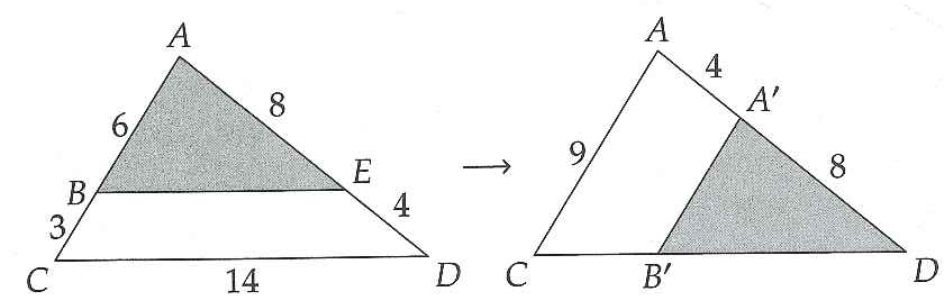
\includegraphics[width=0.7\linewidth]{Geometria/imgs/5_18_aopsgeo_sol2}
	\caption{Solución \ref{ejemplo_5_18_aopsgeo}}
	\label{5_18_aopsgeo_sol2}
\end{figure}

\end{ejemplo}

\textbf{OJO. }Es muy útil \textbf{usar áreas para hallar proporciones}, no solo sirve para calcular áreas de ciertas zonas.

\newpage
\begin{center}
	\vspace{-1cm}
	\subsection{ Ejercicios: Semejanza LLL}
\end{center}
	
\begin{enumerate}
	\item \label{P551_aopgeo_ejercicio} (5.5.1 de \cite{Aops_Geometria}). $X$ e $Y$ están en los lados $\overline{PQ}$ y $\overline{PR}$ de $\triangle PQR$ respectivamente, de forma que $XY \parallel QR$. Si $XY = 5$, $QR=15$ y $YR=8$, encontrar $PY$.
	\item \label{P552_aopgeo_ejercicio} (5.5.2 de \cite{Aops_Geometria}). $[EDC]=25[BFD]$.
			\begin{enumerate}[label=\Alph*)]
				\item Encontrar $\frac{CD}{DB}$.
				\item Encontrar $\frac{[EDC]}{[ABC]}$.
				\item \textbf{Woow} Encontrar $\frac{[AFE]}{[ABC]}$.
			\end{enumerate}
	\begin{figure}[H]
		\centering
		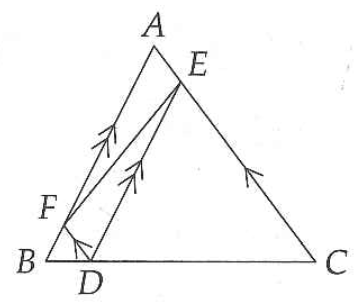
\includegraphics[width=0.4\linewidth]{Geometria/imgs/552_aopgeo_ejer}
		\caption{Ejercicio \ref{P552_aopgeo_ejercicio} }
		\label{552_aopgeo}
	\end{figure}

	\item \label{P553_aopgeo_ejercicio} (5.5.3 de \cite{Aops_Geometria}). En la Figura \ref{553_aopgeo}, $WZ\parallel XY$ y $WX\parallel ZY$, $WA$ y $WB$ intersectan a $XZ$ en $C$ y $D$ respectivamente, de forma que $ZC=XD$.
	\begin{enumerate}[label=\Alph*)]
		\item Probar que $\frac{ZC}{XC} = \frac{AC}{WC}$.
		\item Probar que $\frac{XD}{ZD} = \frac{DB}{WD}$.
		\item Probar que $CD\parallel AB$.
	\end{enumerate}
	\begin{figure}[H]
		\centering
		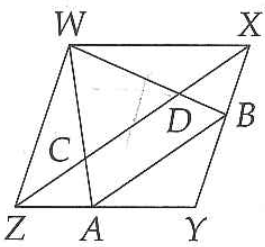
\includegraphics[width=0.3\linewidth]{Geometria/imgs/553_aopgeo_ejer}
		\caption{Ejercicio \ref{P553_aopgeo_ejercicio} }
		\label{553_aopgeo}
	\end{figure}		
	
	\item \label{P554_aopgeo_ejercicio} (5.5.4 de \cite{Aops_Geometria}). En la Figura \ref{554_aopgeo}, $PQ=PR$ y $ZX\parallel QY$
	\begin{enumerate}[label=\Alph*)]
		\item Probar que $\triangle QWZ \sim \triangle RXZ$.
		\item \textbf{Wow} Probar que $YQ = ZX-ZW$.
	\end{enumerate}
	\begin{figure}[H]
		\centering
		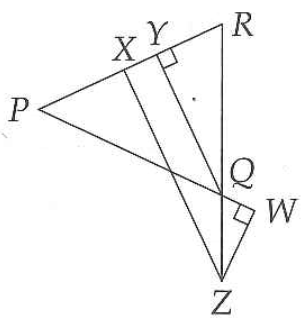
\includegraphics[width=0.3\linewidth]{Geometria/imgs/554_aopgeo_ejer}
		\caption{Ejercicio \ref{P554_aopgeo_ejercicio} }
		\label{554_aopgeo}
	\end{figure}		

	\item \label{P555_aopgeo_ejercicio} (5.5.5 de \cite{Aops_Geometria}). En la Figura \ref{555_aopgeo}, $PA$ y $QB$ son bisectrices de $\angle P$ y $\angle Q$ respectivamente. Si $RX\perp PA$ y $RY\perp BQ$, probar que $XY\parallel PQ$
	\begin{figure}[H]
		\centering
		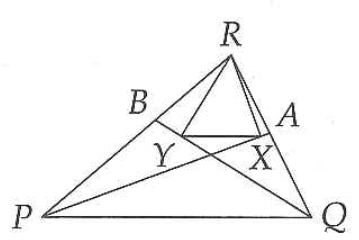
\includegraphics[width=0.3\linewidth]{Geometria/imgs/555_aopgeo_ejer}
		\caption{Ejercicio \ref{P555_aopgeo_ejercicio} }
		\label{555_aopgeo}
	\end{figure}		
	
\end{enumerate}
\newpage

\begin{center}
	\vspace{-1cm}
	\section{ Ejercicios revisión: Semejanza de triángulos}
\end{center}

	\begin{enumerate}
		\item Si dos triángulos son semejantes, probar que las alturas tienen la misma proporción, es decir si la proporción de la semejanza es $k$, entonces la proporción entre las alturas es $k$.
		
		\item Si dos triángulos son semejantes, probar que las medianas tienen la misma proporción, es decir si la proporción de la semejanza es $k$, entonces la proporción entre las medianas es $k$.
		
		\item Si dos triángulos son semejantes, probar que las bisectrices tienen la misma proporción, es decir si la proporción de la semejanza es $k$, entonces la proporción entre las bisectrices es $k$.
		
		\item Si la proporción de la semejanza entre dos triángulos es $k$, entonces la proporción entre las áreas es $k^2$.
		
		\item (Problema 2 Geometría N.2 A.4 de \cite{POTI}). En un $\triangle ABC$, $AB=4cm,BC=5cm$ y $AC=6cm$. Calcular la medida de los lados un triángulo semejante a $ABC$ que tenga perímetro $20cm$.
		
		\item (Problema 3  Geometría N.2 A.4 de \cite{POTI}). Sea $ABC$ un triángulo equilatero de lado $20cm$. Una recta pasa por el punto medio $M$ en el lado $AB$ y un punto $N$ en el lado $AC$ y corta a la recta $\overleftrightarrow{BC}$ en el punto $P$ de modo que $CP=12cm$. Hallar la longitud de $NA$.
		
		%\item (Problema 4  Geometría N.2 A.4 de \cite{POTI}). Sean $D$ y $E$ puntos sobre los lados $AB$ y $AC$ de un triangulo $ABC$ respectivamente. Si
		
		\item \label{review_P522_aopgeo_ejercicio} (5.22 de \cite{Aops_Geometria}). En cada uno de los ejercicios del (a) al (f), mencionar todos los pares de triángulos semejantes posibles y decir por qué lo son.
		\begin{figure}[H]
			\centering
			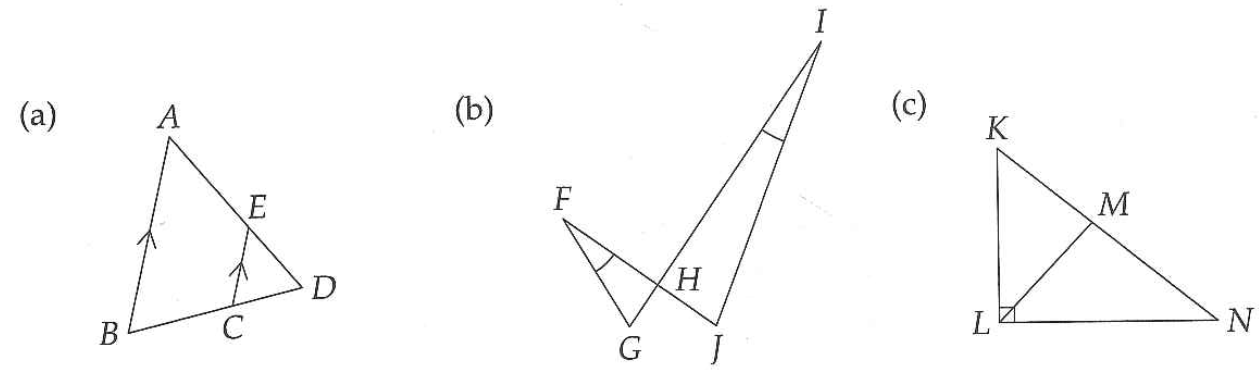
\includegraphics[width=0.9\linewidth]{Geometria/imgs/review_522_1_aopgeo_ejer}
			\label{review_522_1_aopgeo_ejer}
		\end{figure}
		\begin{figure}[H]
			\centering
			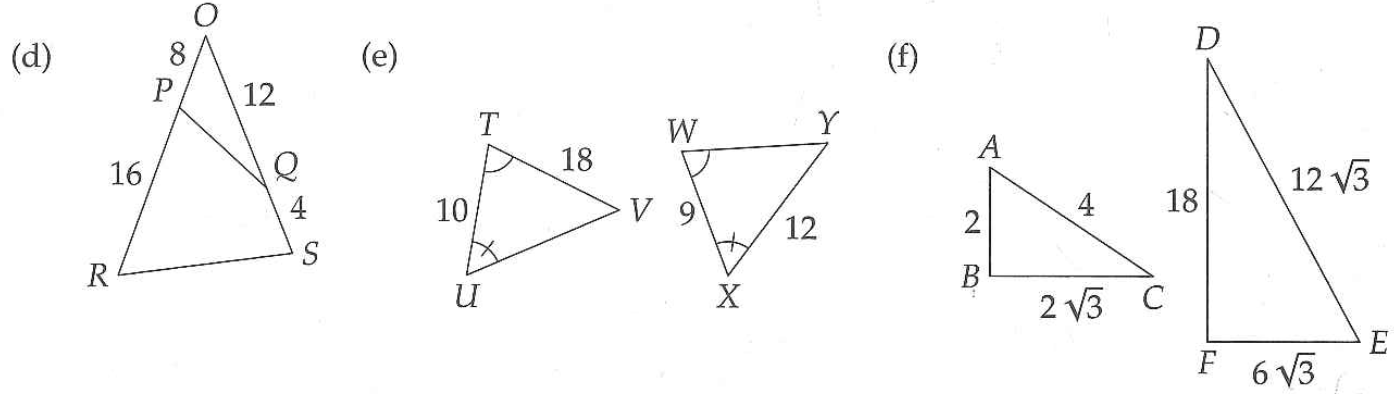
\includegraphics[width=0.9\linewidth]{Geometria/imgs/review_522_2_aopgeo_ejer}
			\label{review_522_2_aopgeo_ejer}
		\end{figure}
		
		\item \label{review_P523_aopgeo_ejercicio} (5.23 de \cite{Aops_Geometria}). En la figura \ref{review_523_aopgeo_ejer}, hallar $x$ e $y$.
			\begin{figure}[H]
				\centering
				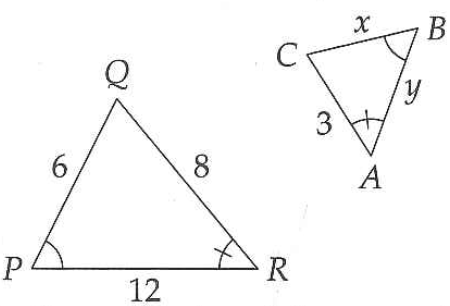
\includegraphics[width=0.4\linewidth]{Geometria/imgs/review_523_aopgeo_ejer}
				\caption{Ejercicio \ref{review_P523_aopgeo_ejercicio}.}
				\label{review_523_aopgeo_ejer}
			\end{figure}
		
		\item \label{review_P524_aopgeo_ejercicio} (5.24 de \cite{Aops_Geometria}). En un $\triangle ABC$, los puntos $P$ y $Q$ están sobre $\overline{AB}$ y $\overline{AC}$ tal que $PQ\parallel BC$. Si $AB=12,PB=9$ y $AC=18$, encontrar $QA$ .
		
		\item \label{review_P525_aopgeo_ejercicio} (5.25 de \cite{Aops_Geometria}). Los lados de un triángulo son 4,6 y 9 centímetros. Uno de los lados de un triángulo similar mide $36cm$. Cuánto es el máximo perimetro que puede tener este otro triángulo?
		
		\item \label{review_P526_aopgeo_ejercicio} (5.26 de \cite{Aops_Geometria}). En la figura \ref{review_523_aopgeo_ejer}, que está mal?
		\begin{figure}[H]
			\centering
			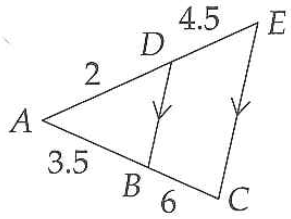
\includegraphics[width=0.35\linewidth]{Geometria/imgs/review_526_aopgeo_ejer}
			\caption{Ejercicio \ref{review_P526_aopgeo_ejercicio}.}
			\label{review_526_aopgeo_ejer}
		\end{figure}
		
		\item \label{review_P527_aopgeo_ejercicio} (5.27 de \cite{Aops_Geometria}). En la figura \ref{review_527_aopgeo_ejer}, hallar $DE$.
		\begin{figure}[H]
			\centering
			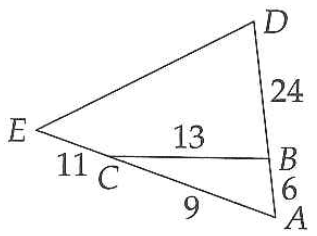
\includegraphics[width=0.3\linewidth]{Geometria/imgs/review_527_aopgeo_ejer}
			\caption{Ejercicio \ref{review_P527_aopgeo_ejercicio}.}
			\label{review_527_aopgeo_ejer}
		\end{figure}
		
		\item \label{review_P528_aopgeo_ejercicio} (5.28 de \cite{Aops_Geometria}). Por qué el diagrama de la figura \ref{review_528_aopgeo_ejer} es imposible?
		\begin{figure}[H]
			\centering
			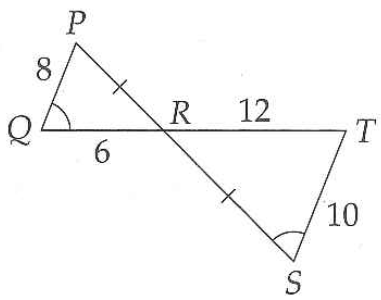
\includegraphics[width=0.4\linewidth]{Geometria/imgs/review_528_aopgeo_ejer}
			\caption{Ejercicio \ref{review_P528_aopgeo_ejercicio}.}
			\label{review_528_aopgeo_ejer}
		\end{figure}
		
		\item \label{review_P529_aopgeo_ejercicio} (5.29 de \cite{Aops_Geometria}). En la figura \ref{review_529_aopgeo_ejer}, hallar $WY$ y $YV$.
		\begin{figure}[H]
			\centering
			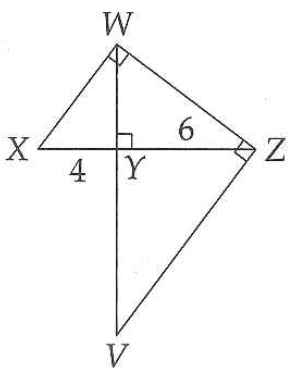
\includegraphics[width=0.3\linewidth]{Geometria/imgs/review_529_aopgeo_ejer}
			\caption{Ejercicio \ref{review_P529_aopgeo_ejercicio}.}
			\label{review_529_aopgeo_ejer}
		\end{figure}
		
		\item \label{review_P530_aopgeo_ejercicio} (5.30 de \cite{Aops_Geometria}). En la figura \ref{review_530_aopgeo_ejer}, $\triangle ABC$ es equilatero.
				\begin{enumerate}[label=\Alph*)]
					\item Probar que $AM=AN$.
					\item Probar que $\triangle AMN$ es equilatero.
				\end{enumerate}
		\begin{figure}[H]
			\centering
			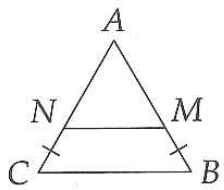
\includegraphics[width=0.28\linewidth]{Geometria/imgs/review_530_aopgeo_ejer}
			\caption{Ejercicio \ref{review_P530_aopgeo_ejercicio}.}
			\label{review_530_aopgeo_ejer}
		\end{figure}
		
		\item \label{review_P531_aopgeo_ejercicio} (5.31 de \cite{Aops_Geometria}). Si $\triangle ABC \sim \triangle YZX$ $[ABC]=40,[YZX]=360,AB=9$ y $BC=12$, hallar:
		\begin{enumerate}[label=\Alph*)]
			\item $YZ$
			\item La longitud de la altura del lado $\overline{XZ}$ del $\triangle YZX$.
		\end{enumerate}
		
		\item \label{review_P532_aopgeo_ejercicio} (5.32 de \cite{Aops_Geometria}). En la figura \ref{review_532_aopgeo_ejer}, $AB=25$ y $BC=12$. Si $AE<BE$ y $\triangle AED \sim \triangle BCE$. Hallar la longitud de $AE$.
		\begin{figure}[H]
			\centering
			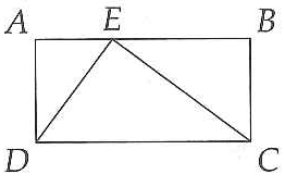
\includegraphics[width=0.35\linewidth]{Geometria/imgs/review_532_aopgeo_ejer}
			\caption{Ejercicio \ref{review_P532_aopgeo_ejercicio}.}
			\label{review_532_aopgeo_ejer}
		\end{figure}
		
		\item \label{review_P533_aopgeo_ejercicio} (5.33 de \cite{Aops_Geometria}). En la figura \ref{review_533_aopgeo_ejer}, $PW=6$ y $WX=4$. Hallar la longitud de $QX$.
		\begin{figure}[H]
			\centering
			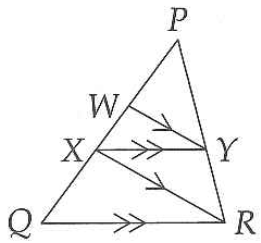
\includegraphics[width=0.35\linewidth]{Geometria/imgs/review_533_aopgeo_ejer}
			\caption{Ejercicio \ref{review_P533_aopgeo_ejercicio}.}
			\label{review_533_aopgeo_ejer}
		\end{figure}
		
		\item \label{review_P534_aopgeo_ejercicio} (5.34 de \cite{Aops_Geometria}). En la figura \ref{review_534_aopgeo_ejer}, $\overline{AP} \parallel \overline{BQ} \parallel \overline{CR}$. Probar que
		\[
				\frac{1}{CR} = \frac{1}{AP} + \frac{1}{BQ}
		\]
		\begin{figure}[H]
			\centering
			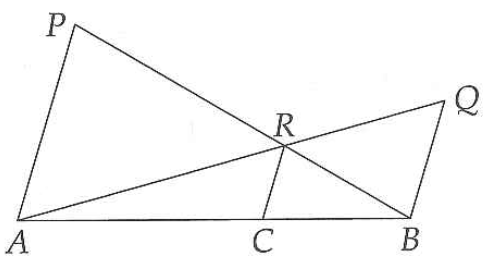
\includegraphics[width=0.45\linewidth]{Geometria/imgs/review_534_aopgeo_ejer}
			\caption{Ejercicio \ref{review_P534_aopgeo_ejercicio}.}
			\label{review_534_aopgeo_ejer}
		\end{figure}
		
		\item \label{review_P535_aopgeo_ejercicio} (5.35 de \cite{Aops_Geometria}). En la figura \ref{review_535_aopgeo_ejer}, dos de los lados del triángulo rectángulo grande miden 20 y12 centímetros. Cuánto mide la altura $h$?
		\begin{figure}[H]
			\centering
			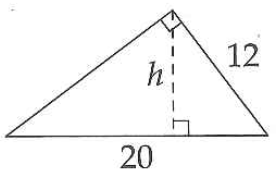
\includegraphics[width=0.4\linewidth]{Geometria/imgs/review_535_aopgeo_ejer}
			\caption{Ejercicio \ref{review_P535_aopgeo_ejercicio}.}
			\label{review_535_aopgeo_ejer}
		\end{figure}
		
		\item \label{review_P536_aopgeo_ejercicio} (5.36 de \cite{Aops_Geometria}). Sea $\triangle ABC$ y sean $D$ y $E$ puntos sobre $\overline{AB}$ y $\overline{AC}$ respectivamente tal que $\overline{DE} \parallel \overline{BC}$. Probar que 
		\[
				\frac{ AD}{AE} = \frac{DB}{CE}
		\]
		
		\item (Tomado de OPM 2017-2018 $2\degree$ eliminatoria, Categoria B problema 2). Sea $\triangle ABC$ de área 9 y $D,E$ y $F$ puntos en los lados $AB, BC$ y $AC$ respectivamente tales que $DE\parallel AC$ y $DF\parallel BC$. Sabiendo que el área de $\triangle DEB$ es cuatro veces el área de $\triangle AFD$, cuál es el área de $\triangle CFE$?	
			\begin{figure}[H]
				\centering
				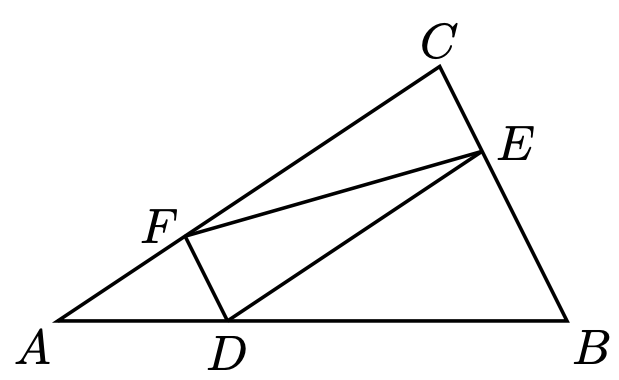
\includegraphics[width=0.45\linewidth]{Geometria/imgs/AV_P4}
				%\caption{}
				\label{avp4}
			\end{figure}
	\end{enumerate}
\newpage

\begin{center}
	\vspace{-1cm}
	\section{ Ejercicios revisión avanzados: Semejanza de triángulos}
\end{center}
\begin{enumerate}
	\item \label{challege_537_aopgeo_ejercicio} (5.37 de \cite{Aops_Geometria}). Sea $ABC$ un triángulo, y sean los puntos $D$ y $E$ sobre $\overline{AB}$ y $\overline{AC}$ respectivamente tales que $\frac{AD}{AE}=\frac{BD}{CE}$. Probar que $\overline{DE} \parallel \overline{BC}$.
	
	\item \label{challege_539_aopgeo_ejercicio}(5.39 de \cite{Aops_Geometria}). En la figura \ref{challege_539_aopgeo_ejer}, $\triangle ABC$ es isosceles, $CH=24cm$, $DE=GF,HF=12cm$ y $FB=6cm$. Encontrar el área de $CDEFG$.
	\begin{figure}[H]
		\centering
		\includegraphics[width=0.4\linewidth]{Geometria/imgs/challege_539_aopgeo_ejer}
		\caption{Ejercicio \ref{challege_539_aopgeo_ejercicio}.}
		\label{challege_539_aopgeo_ejer}
	\end{figure}

	\item \label{challege_540_aopgeo_ejercicio}(5.40 de \cite{Aops_Geometria}). En la figura \ref{challege_540_aopgeo_ejer}, $AD\cdot AC =AE\cdot AB$. Probar que $\angle CDE + \angle CBE = 180\degree$ y $\angle ADB + \angle BEC = 180\degree$.
	\begin{figure}[H]
		\centering
		\includegraphics[width=0.3\linewidth]{Geometria/imgs/challege_540_aopgeo_ejer}
		\caption{Ejercicio \ref{challege_540_aopgeo_ejercicio}.}
		\label{challege_540_aopgeo_ejer}
	\end{figure}
	
	\item \label{challege_541_aopgeo_ejercicio}(5.41 de \cite{Aops_Geometria}). $D,E$ y $F$ están en los lados $\overline{BC}$, $\overline{AC}$ y $\overline{AB}$ recpectivamente del triángulo $ABC$, de forma que $\overline{DE} \parallel \overline{AB}$, $\overline{DF} \parallel \overline{AC}$ y $\overline{BC} \parallel \overline{EF}$. Probar que $D,E$ y $F$ son puntos medios de los lados de $\triangle ABC$.
	
	\item \label{challege_542_aopgeo_ejercicio}(5.42 de \cite{Aops_Geometria}). En la figura \ref{challege_542_aopgeo_ejer}, $\overline{PS} \parallel \overline{QT}$ y $\overline{PQ} \parallel \overline{ST}$. Probar que $\frac{SU}{SP}=\frac{QP}{QR}$.
	\begin{figure}[H]
		\centering
		\includegraphics[width=0.3\linewidth]{Geometria/imgs/challege_542_aopgeo_ejer}
		\caption{Ejercicio \ref{challege_542_aopgeo_ejercicio}.}
		\label{challege_542_aopgeo_ejer}
	\end{figure}

	\item \label{challege_543_aopgeo_ejercicio}(5.43 de \cite{Aops_Geometria}). En la figura \ref{challege_543_aopgeo_ejer}, $[XYZ] = 8$. Los puntos $A$ y $B$ son puntos medios de los segmentos congruentes $\overline{XY}$ y $\overline{XZ}$. La altura $\overline{XC}$ biseca a $\overline{YZ}$. Cuál es el área de la región sombreada?
	\begin{figure}[H]
		\centering
		\includegraphics[width=0.4\linewidth]{Geometria/imgs/challege_543_aopgeo_ejer}
		\caption{Ejercicio \ref{challege_543_aopgeo_ejercicio}.}
		\label{challege_543_aopgeo_ejer}
	\end{figure}

	\item \label{challege_544_aopgeo_ejercicio}(5.44 de \cite{Aops_Geometria}). Al unir los puntos medios de los lados de un triangulo equilatero se construye un segundo triángulo. Un tercer triángulo es construido uniendo los puntos medios de los lados del segundo triángulo. Este proceso se repite hasta construir el décimo triángulo. Cuál es la razón entre las área del décimo triángulo y el tercer triángulo?
	
	\item \label{challege_545_aopgeo_ejercicio}(5.45 de \cite{Aops_Geometria}). En la figura \ref{challege_545_aopgeo_ejer}, $ABCD$ es un rectángulo, $AB=5$ y $BC=3$, $FG=1$ y $GC=2$ . Encontrar el área de $\triangle AEB$.
	\begin{figure}[H]
		\centering
		\includegraphics[width=0.3\linewidth]{Geometria/imgs/challege_545_aopgeo_ejer}
		\caption{Ejercicio \ref{challege_545_aopgeo_ejercicio}.}
		\label{challege_545_aopgeo_ejer}
	\end{figure}

	\item \label{challege_546_aopgeo_ejercicio}(5.46 de \cite{Aops_Geometria}). \textbf{Wow}. En la figura \ref{challege_546_aopgeo_ejer}, $AC=4$ y $BC=3$, $AB=5$ y $\angle ACB=90\degree$ . La secuencia infinita de puntos $C_1,C_2,C_3,C_4\dots$ se forma de la siguiente manera: $C_1$ es el pie de la altura de $C$ sobre $AB$, $C_2$ es el pie de la altura de $C_1$ sobre $AC$, $C_3$ es el pie de la altura de $C_2$ sobre $AB$, y así sucesivamente. Calcular la suma
	\[
			\overline{CC_1} + \overline{C_1C_2}+ \overline{C_2C_3} + \dots 
	\]
	\begin{figure}[H]
		\centering
		\includegraphics[width=0.4\linewidth]{Geometria/imgs/challege_546_aopgeo_ejer}
		\caption{Ejercicio \ref{challege_546_aopgeo_ejercicio}.}
		\label{challege_546_aopgeo_ejer}
	\end{figure}

	\item \label{challege_547_aopgeo_ejercicio}(5.47 de \cite{Aops_Geometria}). \textbf{Wow}. En la figura \ref{challege_547_aopgeo_ejer}, el triángulo grande es equilatero y sus lados se dividen en 4 segmentos congruentes para construir los triángulos equilateros pequeños que se encuentran en el interior. Considere ahora que no se divide en 4 sino en $n$ segmentos congruentes para construir triángulos equilateros pequeños en el interior. Use esto para probar que la suma de los primeros $n$ números impares es $n^2$.
	\begin{figure}[H]
		\centering
		\includegraphics[width=0.3\linewidth]{Geometria/imgs/challege_547_aopgeo_ejer}
		\caption{Ejercicio \ref{challege_547_aopgeo_ejercicio}.}
		\label{challege_547_aopgeo_ejer}
	\end{figure}

	\item \label{challege_548_aopgeo_ejercicio}(5.48 de \cite{Aops_Geometria}). \textbf{Wow}. En la figura \ref{challege_548_aopgeo_ejer}, $AB=6,CD=8,BC=DA=2$ y $\overline{AB} \parallel \overline{CD}$. $P$ es punto medio de $\overline{AB}$, $\overline{PR} \parallel \overline{BC}$ y $\overline{PQ} \parallel \overline{AD}$. Calcular $\frac{PX}{YR}$
	\begin{figure}[H]
		\centering
		\includegraphics[width=0.4\linewidth]{Geometria/imgs/challege_548_aopgeo_ejer}
		\caption{Ejercicio \ref{challege_548_aopgeo_ejercicio}.}
		\label{challege_548_aopgeo_ejer}
	\end{figure}

	\item \label{challege_549_aopgeo_ejercicio}(5.49 de \cite{Aops_Geometria}). \textbf{Wow}. En la figura \ref{challege_549_aopgeo_ejer}, $AF=FG=GB$ y $E$ es punto medio de $\overline{DC}$. $[ABCD]=70$. Hallar el área de $\triangle AHF$.
	\begin{figure}[H]
		\centering
		\includegraphics[width=0.4\linewidth]{Geometria/imgs/challege_549_aopgeo_ejer}
		\caption{Ejercicio \ref{challege_549_aopgeo_ejercicio}.}
		\label{challege_549_aopgeo_ejer}
	\end{figure}

	\item \label{challege_551_aopgeo_ejercicio}(5.51 de \cite{Aops_Geometria}). \textbf{Wow}. En la figura \ref{challege_551_aopgeo_ejer},  $\overline{BC} \parallel \overline{UR}$, $\overline{PS} \parallel \overline{BA}$ y $\overline{TQ} \parallel \overline{AC}$. Probar que
	\[
			\frac{PQ}{BC} + \frac{RS}{CA} + \frac{TU}{AB} = 1
	\]
			\begin{figure}[H]
				\centering
				\includegraphics[width=0.4\linewidth]{Geometria/imgs/challege_551_aopgeo_ejer}
				\caption{Ejercicio \ref{challege_551_aopgeo_ejercicio}.}
				\label{challege_551_aopgeo_ejer}
			\end{figure}
	
	\item (Problema 3 Avanzado OMAPA 2012). 
			\begin{figure}[H]
				\centering
				\includegraphics[width=\linewidth]{Geometria/imgs/OMAPA_AV_2012_P3}
				%\caption{Ejercicio \ref{challege_551_aopgeo_ejercicio}.}
				\label{OMAPA_AV_2012_P3}
			\end{figure}
	
	\item (UK Math Trust Problem of the day 58). En la Figura \ref{UK58} se muestran dos circulos cuyos radios son 3 y 9 unidades, y cuyos centros estan a una distancia de 20 unidades. El segmento $\overline{PQ}$ es tangente a ambos circulos. Cuánto mide $PQ$?
	
			\begin{figure}[H]
				\centering
				\includegraphics[width=0.5\linewidth]{Geometria/imgs/UKMathTrust_PrblemOfTheDay_58}
				%\caption{Ejercicio \ref{challege_551_aopgeo_ejercicio}.}
				\label{UK58}
			\end{figure}
		
	\item (UK Math Trust Problem of the day 66). En la Figura \ref{UK58} calcular el área de toda la figura.
	
	\begin{figure}[H]
		\centering
		\includegraphics[width=0.5\linewidth]{Geometria/imgs/UKMathTrust_PrblemOfTheDay_66}
		%\caption{Ejercicio \ref{challege_551_aopgeo_ejercicio}.}
		\label{UK66}
	\end{figure}

\item (Fase clasificatoria Nivel Avanzado UdeA). 
		\begin{figure}[H]
			\centering
			\includegraphics[width=0.95\linewidth]{Geometria/imgs/udeaproblemasemejanza1}
			%\caption{Ejercicio \ref{challege_551_aopgeo_ejercicio}.}
			%\label{udea1}
		\end{figure}
\end{enumerate}
\newpage


\chapter{Circulos y angulos}
\newpage


\begin{center}
	\vspace{-1cm}
	\section{ Ejercicios: Circulos y ángulos}
\end{center}

\begin{enumerate}	
	\item (Problema 5  Geometría N.2 A.4 de \cite{POTI}). Considere la cricunferencia que circunscribe al triángulo $ABC$. Sea $AE$ un diámetro de esta circunferencia y $AD$ la altura del triángulo en el vértice $A$. Si $AB=6,AC=10$ y $AE=30$. Hallar cuánto mide $AD$.
\end{enumerate}

\newpage
